% This document is based on a template created by Ted Pavlic (http://www.tedpavlic.com)


%----------------------------------------------------------------------------------------
%	PACKAGES AND OTHER DOCUMENT CONFIGURATIONS
%----------------------------------------------------------------------------------------

\documentclass{article}

\usepackage{fancyhdr} % Required for custom headers
\usepackage{lastpage} % Required to determine the last page for the footer
\usepackage{extramarks} % Required for headers and footers
\usepackage[usenames,dvipsnames]{color} % Required for custom colors
\usepackage{graphicx} % Required to insert images
\usepackage{subcaption}
\usepackage{listings} % Required for insertion of code
\usepackage{courier} % Required for the courier font
%\usepackage{lipsum} % Used for inserting dummy 'Lorem ipsum' text into the template
\usepackage{amsmath,siunitx,physics,amssymb}
\usepackage{placeins}
\usepackage{enumitem}
\usepackage{minted,listings}
\usepackage{hyperref,cleveref}

% Margins
\topmargin=-0.45in
\evensidemargin=0in
\oddsidemargin=0in
\textwidth=6.5in
\textheight=9.0in
\headsep=0.25in

\linespread{1.1} % Line spacing

% Set up the header and footer
\pagestyle{fancy}
\lhead{\hmwkAuthorName} % Top left header
\chead{\hmwkClass\ : \hmwkTitle} % Top center head
%\rhead{\firstxmark} % Top right header
\lfoot{\lastxmark} % Bottom left footer
\cfoot{} % Bottom center footer
\rfoot{Page\ \thepage\ of\ \protect\pageref{LastPage}} % Bottom right footer
\renewcommand\headrulewidth{0.4pt} % Size of the header rule
\renewcommand\footrulewidth{0.4pt} % Size of the footer rule

%\setlength\parindent{0pt} % Removes all indentation from paragraphs

%----------------------------------------------------------------------------------------
%	DOCUMENT STRUCTURE COMMANDS
%	Skip this unless you know what you're doing
%----------------------------------------------------------------------------------------

% Header and footer for when a page split occurs within a problem environment
\newcommand{\enterproblemHeader}[1]{
%\nobreak\extramarks{#1}{#1 continued on next page\ldots}\nobreak
%\nobreak\extramarks{#1 (continued)}{#1 continued on next page\ldots}\nobreak
}

% Header and footer for when a page split occurs between problem environments
\newcommand{\exitproblemHeader}[1]{
%\nobreak\extramarks{#1 (continued)}{#1 continued on next page\ldots}\nobreak
%\nobreak\extramarks{#1}{}\nobreak
}

\setcounter{secnumdepth}{0} % Removes default section numbers
\newcounter{problem} % Creates a counter to keep track of the number of problems
\setcounter{problem}{-1}

\newcommand{\problemName}{}
\newenvironment{problem}[1][Part \theproblem]{ % Makes a new environment called problem which takes 1 argument (custom name) but the default is "problem #"
	\stepcounter{problem} % Increase counter for number of problems
	\renewcommand{\problemName}{#1} % Assign \problemName the name of the problem
	\section{\problemName} % Make a section in the document with the custom problem count
	\enterproblemHeader{\problemName} % Header and footer within the environment
}{
	\exitproblemHeader{\problemName} % Header and footer after the environment
}

\newcommand{\problemAnswer}[1]{ % Defines the problem answer command with the content as the only argument
	\noindent\framebox[\columnwidth][c]{\begin{minipage}{0.98\columnwidth}#1\end{minipage}} % Makes the box around the problem answer and puts the content inside
}

\newcounter{subproblem}[problem]
\newcommand{\subproblemName}{}
\newenvironment{subproblem}[1][\theproblem~(\alph{subproblem})]{ % New environment for sections within  problems, takes 1 argument - the name of the section
	\stepcounter{subproblem}
	\renewcommand{\subproblemName}{#1} % Assign \problemName the name of the problem
	\subsection{\subproblemName} % Make a section in the document with the custom problem count
	\enterproblemHeader{\subproblemName} % Header and footer within the environment
}{
	\enterproblemHeader{\problemName} % Header and footer after the environment
}

\newcommand{\numberthis}{\addtocounter{equation}{1}\tag{\theequation}}

%----------------------------------------------------------------------------------------
%	NAME AND CLASS SECTION
%----------------------------------------------------------------------------------------

\newcommand{\hmwkTitle}{Assignment\ \#$4$} % Assignment title
\newcommand{\hmwkDueDate}{Moday,\ April\ 2,\ 2018} % Due date
\newcommand{\hmwkClass}{CSC411} % Course/class
\newcommand{\hmwkClassTime}{} % Class/lecture time
\newcommand{\hmwkAuthorName}{Izaak Niksan and Lukas Zhornyak} % Your name

%----------------------------------------------------------------------------------------
%	TITLE PAGE
%----------------------------------------------------------------------------------------

\title{
	\vspace{2in}
	\textmd{\textbf{\hmwkClass:\ \hmwkTitle}}\\
	\normalsize\vspace{0.1in}\small{Due\ on\ \hmwkDueDate}\\
	\vspace{0.1in}
	\vspace{3in}
}

\author{\textbf{\hmwkAuthorName}}
%\date{} % Insert date here if you want it to appear below your name

%----------------------------------------------------------------------------------------

\begin{document}

\maketitle
\clearpage

%----------------------------------------------------------------------------------------
%	ENVIRONMENT
%----------------------------------------------------------------------------------------

\begin{problem}[Environment]	
	This project was created with Python 3.6.4 with numpy 1.14.1, scipy 1.0.0, scikit-image 0.13.1, and matplotlib 2.1.2, pytorch 0.3.0, torchvision 0.2.0, as well as all associated dependencies.
\end{problem}
\clearpage

%----------------------------------------------------------------------------------------
%	PART 1
%----------------------------------------------------------------------------------------
\FloatBarrier
\begin{problem}
	By inspecting the code it was determined that the grid is represented by a numpy array of 9 elements, one for each space on the board; 0 represents an empty space, 1 represents the presence of an x in the space, and 2 represents the presence of an o in the space. The parameter \texttt{turn} represents whose turn it is, taking on values of 1 or 2 (for x and o respectively). The parameter \texttt{done} is a Boolean value denoting whether or not the game is finished.
	
	A game of Tic-Tac-Toe (albeit an amateur one) was simulated using the code seen in \cref{lst:1}. Its text output is seen below it.
	\begin{listing}
		\caption{Simulated game of Tic-Tac-Toe.}
		\label{lst:1}
		\begin{minted}[mathescape, linenos, numbersep=5pt, gobble=3, frame=lines, framesep=2mm, tabsize=4, breaklines]{python}
			p1_env=Environment()
			print('First turns:')
			p1_env.step(0)
			p1_env.step(1)
			p1_env.render()
			print('Second turns:')
			p1_env.step(8)
			p1_env.step(5)
			p1_env.render()
			print('Third turn (x wins):')
			p1_env.step(4)
			p1_env.render()
		\end{minted}
		\begin{verbatim}
			First turns:
			xo.
			...
			...
			====
			Second turns:
			xo.
			..o
			..x
			====
			Third turn (x wins):
			xo.
			.xo
			..x
			====
		\end{verbatim}
	\end{listing}	
	
\end{problem}
\clearpage

%----------------------------------------------------------------------------------------
%	PART 2
%----------------------------------------------------------------------------------------
\FloatBarrier
\begin{problem}
	
\begin{subproblem}
	The completed policy class is shown in \cref{lst:2a}.
	\begin{listing}
		\caption{Completed Policy class.}
		\label{lst:2a}
		\begin{minted}[mathescape, linenos, numbersep=5pt, gobble=3, frame=lines, framesep=2mm, tabsize=4, breaklines]{python}
			class Policy(nn.Module):		
				def __init__(self, input_size=27, hidden_size=64, output_size=9):
				super(Policy, self).__init__()
				self.policy = nn.Sequential(
					nn.Linear(input_size, hidden_size),
					nn.ReLU(),
					nn.Linear(hidden_size, output_size),
					nn.Softmax(1)
				)
				def forward(self, x):
					return self.policy.forward(x)
		\end{minted}
	\end{listing}
\end{subproblem}
	
\begin{subproblem}
	By inspecting the code in the \texttt{select\_action} function, it was determined that the 27-dimensional array is used to one-hot encode the state of the board. In other words, three rows are used to represent the locations of an empty, x, or o element respectively. \Cref{lst:2b} shows a numpy \texttt{grid} array and its corresponding \texttt{torch.FloatTensor}.

	\begin{listing}
		\caption{Representation of the 27-dimensional array.}
		\label{lst:2b}
		\begin{minted}[mathescape, linenos, numbersep=5pt, gobble=3, frame=lines, framesep=2mm, tabsize=4, breaklines]{python}
			import tictactoe  
			
			state=np.array([0,1,2]*3)
			print('The grid array format is:')
			print(state)
			state = torch.from_numpy(state).long().unsqueeze(0)
			state = torch.zeros(3,9).scatter_(0,state,1)
			print('\nThe 27-dimensional array format is:')
			print(state)
		\end{minted}
		\begin{verbatim}
		The grid array format is:
		[0 1 2 0 1 2 0 1 2]
		
		The 27-dimensional array format is:
		
		1     0     0     1     0     0     1     0     0
		0     1     0     0     1     0     0     1     0
		0     0     1     0     0     1     0     0     1
		[torch.FloatTensor of size 3x9]
		\end{verbatim}
	\end{listing}
\end{subproblem}
	
\begin{subproblem}
	The output of this policy is a 9-dimensional vector, in the same format as \texttt{grid} described in Part 1, with each value representing the probability of that spot being chosen this turn. In other words, it represents a discrete probability distribution. Since \texttt{select\_action} takes a sample from this distribution, and does not always choose the element of highest probability, the policy is therefore stochastic.
\end{subproblem}
	
\end{problem}
\clearpage

%----------------------------------------------------------------------------------------
%	PART 3
%----------------------------------------------------------------------------------------
\FloatBarrier
\begin{problem}
	\begin{subproblem}
		The completed \texttt{compute\_returns} function is shown in \cref{lst:3a}.
		\begin{listing}
			\caption{Reward Values.}
			\label{lst:3a}
			\begin{minted}[mathescape, linenos, numbersep=5pt, gobble=4, frame=lines, framesep=2mm, tabsize=4, breaklines]{python}
				def compute_returns(rewards, gamma=1.0):
					v = list(accumulate([r * gamma ** i for i, r in enumerate(rewards)][::-1]))
					return [r / gamma ** i for i, r in enumerate(v[::-1])]
			\end{minted}
		\end{listing}
	\end{subproblem}
	
	\begin{subproblem}
The reason why a backward pass cannot be computed before the entire episode is completed is because the \textit{compute\_returns} function requires actions for all values of t in order for it to compute the total return. Thus, computing it midway through would not be possible as the reward would depend on actions in the future. Furthermore, even if one were to restructure the code to allow for computing the rewards before the end of an episode, the problem of improperly-scaled rewards may also arise. In other words, more recent actions should be weighed more strongly than older ones by an exponentiated gamma factor; changing the model to be rewarded midway through leads to a situtation where it is not immediately clear how to properly account for a time-dependent reward system. Finally, by the very nature of the way this algorithm was constructed, computing a backward pass midway is not advisable since during an actual play-through no further training will be done. The model at testing time is to remain static.
	\end{subproblem}
	
\end{problem}
\clearpage

%----------------------------------------------------------------------------------------
%	PART 4
%----------------------------------------------------------------------------------------
\FloatBarrier
\begin{problem}
	
\begin{subproblem}
	The modified \texttt{get\_rewards} function is seen in \cref{lst:4a}
	\begin{listing}
		\caption{Reward Values.}
		\label{lst:4a}
		\begin{minted}[mathescape, linenos, numbersep=5pt, gobble=3, frame=lines, framesep=2mm, tabsize=4, breaklines]{python}
			def get_reward(status):
				"""Returns a numeric given an environment status."""
				return {
					Environment.STATUS_VALID_MOVE  : 0,
					Environment.STATUS_INVALID_MOVE: -0.5,
					Environment.STATUS_WIN         : 1,
					Environment.STATUS_TIE         : 0,
					Environment.STATUS_LOSE        : -1
				}[status]
		\end{minted}
	\end{listing}
\end{subproblem}

\begin{subproblem}
	It was decided that the only positive reward should be winning a game. It yields a reward of 1. The justification for this decision is that ultimately the algorithm is attempting to win games, and thus is rewarded for doing so.
	
	Making a valid move and tying a game yield rewards of 0. Since these actions do not explicitly work towards winning games, but also are not unfavourable, no reward is associated with them.
	
	Invalid moves and losing a game are assigned reward values of \num{-0.5} and \num{-1} respectively. Making an invalid move is unwanted since it effectively skips the player's turn. An efficient algorithm should not make invalid moves. Losing a game is clearly unwanted, and thus its reward is the most negative of all actions.		
\end{subproblem}
	
\end{problem}
\clearpage

%----------------------------------------------------------------------------------------
%	PART 5
%----------------------------------------------------------------------------------------
\FloatBarrier
\begin{problem}
\begin{subproblem}
	The training curve obtained during training is shown in \cref{fig:5a}. Beyond the choice of the number of hidden units and tweaking the returns from Part 4, no additional hyperparameters were tuned. The original choice for returns did not place enough penalty on invalid moves, leading to suboptimal performance.
	\begin{figure}
		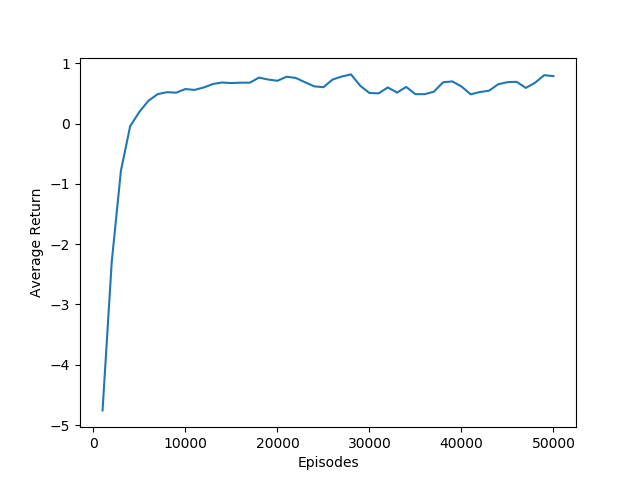
\includegraphics[width=\linewidth]{training_curve}
		\caption{Average return versus episodes elapsed during training of policy.}
		\label{fig:5a}
	\end{figure}
\end{subproblem}

\begin{subproblem}
	The policy was trained with 32, 64, and 128 hyperparameters with the final trained policies compared via their win rates against a random opponent. Each choice was trained several times to reduce the impact of random chance on the final performance. The results obtained are shown in \cref{tab:5b}. 
	
	Across the different trials, there seems to be a very large margin in the obtained results, greater than the difference between the choice of different hidden layer sizes. However, a policy based around a hidden layer size of 32 seems to consistently provide the best performance and so was chosen for further experimentation.
	\begin{table}
		\caption{Win rate across several trails for a policy models with 32, 64, or 128 hidden units.}
		\label{tab:5b}
		\centering
		\begin{tabular}{c S S S}
			Trial & {32 Hidden Units} & {64 Hidden Units} & {128 Hidden Units} \\
			\hline
			1 & 0.814 & 0.782 & 0.837 \\
			2 & 0.862 & 0.866 & 0.722 \\
			3 & 0.867 & 0.871 & 0.756 \\
			4 & 0.821 & 0.674 & 0.767 \\
			5 & 0.804 & 0.745 & 0.743 \\
			\hline
		\end{tabular}
	\end{table}
\end{subproblem}
	
\begin{subproblem}
	To determine the approximate episode when the model learned to stop playing invalid moves, the average number of invalid moves made as the training progressed was plotted. This is shown in \cref{fig:5c}. 
	\begin{figure}
		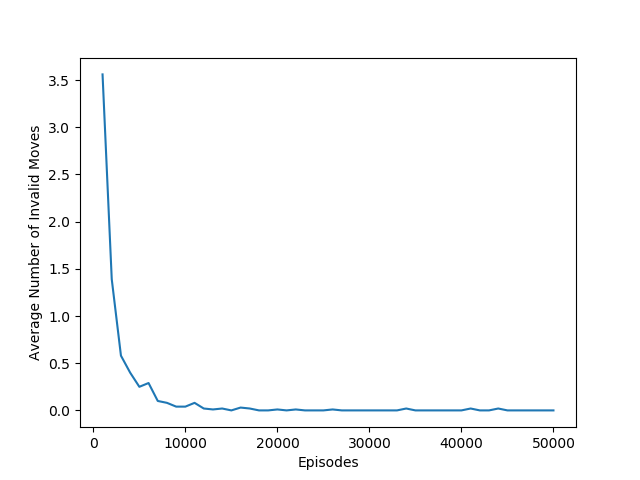
\includegraphics[width=\linewidth]{invalid_moves}
		\caption{Average number of invalid moves across one hundred games versus number of episodes elapsed during training.}
		\label{fig:5c}
	\end{figure}
\end{subproblem}
	
\begin{subproblem}
	Across one hundred games, the model managed to win 81, lose 14, and tie 5. Five games are shown in \cref{lst:5d}. 
	
	The most noticeable strategy exhibited by the policy is to prioritize the diagonal, with diagonals being the source of the majority of its victories. Another may be prioritizing the centre as the games usually end with the centre filled by x. Both these may be the result of an attempt to control as large a territory as possible to limit the ability of the opponent to win. 
	\begin{listing}
		\caption{Five example games from fully trained policy.}
		\label{lst:5d}
		\centering
		\begin{minipage}[t]{0.1\linewidth}
			\begin{verbatim}
				..x
				o..
				...
				====
				..x
				ox.
				.o.
				====
				..x
				ox.
				xo.
				====
			\end{verbatim}
		\end{minipage}%
		\begin{minipage}[t]{0.1\linewidth}
			\begin{verbatim}
				.o.
				...
				..x
				====
				.ox
				...
				o.x
				====
				xox
				o..
				o.x
				====
				xox
				ox.
				o.x
				====
			\end{verbatim}
		\end{minipage}%
		\begin{minipage}[t]{0.1\linewidth}
			\begin{verbatim}
				..o
				.x.
				...
				====
				..o
				ox.
				..x
				====
				..o
				oxo
				x.x
				====
				x.o
				oxo
				x.x
				====
			\end{verbatim}
		\end{minipage}%
		\begin{minipage}[t]{0.1\linewidth}
			\begin{verbatim}
				o..
				...
				..x
				====
				o.x
				..o
				..x
				====
				o.x
				.xo
				o.x
				====
				oox
				.xo
				oxx
				====
				oox
				xxo
				oxx
				====
			\end{verbatim}
		\end{minipage}%
		\begin{minipage}[t]{0.1\linewidth}
			\begin{verbatim}
				..x
				...
				o..
				====
				.ox
				.x.
				o..
				====
				xox
				.x.
				oo.
				====
				xox
				.x.
				oox
				====
			\end{verbatim}
		\end{minipage}%
	\end{listing}
\end{subproblem}
	
\end{problem}
\clearpage

%----------------------------------------------------------------------------------------
%	PART 6
%----------------------------------------------------------------------------------------
\FloatBarrier
\begin{problem}
	
	
\end{problem}
\clearpage

%----------------------------------------------------------------------------------------
%	PART 7
%----------------------------------------------------------------------------------------
\FloatBarrier
\begin{problem}
	
	
\end{problem}
\clearpage

%----------------------------------------------------------------------------------------
%	PART 8
%----------------------------------------------------------------------------------------
\FloatBarrier
\begin{problem}
	
	
\end{problem}
\clearpage


%----------------------------------------------------------------------------------------

\end{document}